% MAE 249 Mini-Project Report template (N = 1 student -> max 3 pages)
% Format: letter, Times (mathptmx), 12 pt, 1" margins, single-spaced, single column.
% Captions / in-figure text: >= 10 pt.
\documentclass[12pt,letterpaper]{article}
\usepackage[margin=1in]{geometry}
\usepackage{mathptmx}
\usepackage{graphicx,booktabs,amsmath}
\usepackage{tikz}\usetikzlibrary{positioning, arrows.meta}
\usepackage[font=small,labelfont=bf]{caption} % small = 10.95pt at 12pt base (>= 10 pt)
\usepackage[hidelinks]{hyperref}
\usepackage{setspace}\singlespacing
\setlength{\parindent}{0pt}\setlength{\parskip}{2pt}
\usepackage{titlesec}
\titleformat{\section}{\bfseries\normalsize}{\thesection.}{0.5em}{}
\titlespacing*{\section}{0pt}{4pt}{1pt}
\newcommand{\meff}{\mu_{\mathrm{eff}}}

\title{\vspace{-2em}\large\textbf{Wall-Thickness Tolerance vs.\ Modulus Uncertainty in a Fiber-Reinforced Bending Actuator Model}\vspace{-0.5em}}
\author{Chengen Ruan \\ MAE 249 Soft Robotics, UC San Diego \\ Mini-Project Report, November 24, 2026}
\date{}

\begin{document}
\maketitle
\vspace{-1.5em}

\section{Research Question}
The analytical model of Polygerinos et al.~\cite{poly2015} gives the pressure $P(\theta)$ a fiber-reinforced bending actuator needs to reach a bending angle $\theta$. At $360^\circ$ it reproduces the measured 207~kPa only with a calibrated modulus $\meff=0.314$~MPa, 43\% above the small-strain value $2C_1=0.22$~MPa. A Yeoh material model and the outer sheath can remove part of the difference; the rest is a \emph{systematic bias} (gap $=P_{\exp}-P_{\rm model}$). Wall thickness varies randomly from part to part and enters the model strongly. \textbf{Question:} after Yeoh and sheath corrections, is the remaining gap larger or smaller than the pressure scatter caused by wall-thickness tolerance? Because bias and scatter are different kinds of quantity, I define the crossover $\sigma_t^*$ as the $\sigma_t$ at which the $1\sigma$ pressure scatter equals $|\text{gap}|$. \textbf{Hypothesis:} below $\sigma_t^*$ modulus/model bias matters more, above it thickness tolerance matters more. Against the measured tolerance of 0.04--0.06~mm: $\sigma_t^*$ lies \emph{above} that band after Yeoh alone (bias dominates) and \emph{below} it for a suitable sheath (tolerance dominates). \textbf{Caveat:} my model gives 237.8~kPa at $360^\circ$, 8\% above the paper's analytical 220~kPa, unexplained (Sec.~4); the gap may thus include an implementation difference.

\section{Approach}
\textbf{Model.} I vectorized the course notebook implementation of $P(\theta)=M(\theta)/\kappa$, $\kappa=(4a^3+3\pi a^2 b)/6$, with axial stretch $\lambda=r\theta/L+1$, using Gauss--Legendre quadrature (order 32; 12 for Monte Carlo), matching the notebook's \texttt{scipy.quad} to $10^{-13}$~kPa. Baseline $a,b,t,L=8,2,2,160$~mm. Neo-Hookean wall: $s=\mu(\lambda-\lambda^{-3})$. Yeoh wall: $s=2(\lambda-\lambda^{-3})\,[C_1+2C_2(I_1-3)]$ with $I_1=\lambda^2+1+\lambda^{-2}$ (plane-strain form matching $\lambda-\lambda^{-3}$), $C_1{=}0.11$, $C_2{=}0.02$~MPa.\par\textbf{Sheath and equivalent shift.} an added 1~mm Neo-Hookean layer on the top wall ($\tau\in[t,t{+}1]$) with $\mu_s=25$, 39, 92~kPa; 39~kPa was solved to reproduce an earlier estimate of 211.7~kPa and is not taken from a datasheet. The equivalent modulus shift is $\Delta\mu_{\rm eq}=\Delta P/(dP/d\mu)_{\rm NH}$ with $(dP/d\mu)_{\rm NH}=757$~kPa/MPa at $360^\circ$.\par\textbf{Sensitivity and Monte Carlo.} Elasticities are $\pm1\%$ central differences of $\ln P$ in $\ln x$, $x\in\{a,b,t,L,\mu\}$. Because the scatter is nearly linear in $\sigma_t$, $\sigma_t^*\simeq|\text{gap}|\,t/(\varepsilon_t P)$ with $\varepsilon_t=d\ln P/d\ln t$; the Monte Carlo checks this and adds what a linearization about the nominal $t$ does not contain (the correlated $a$ shift and the independent $a,b,L$ floor). Setup: $t\sim\mathcal N(2,\sigma_t^2)$, 25 log-spaced $\sigma_t\in[0.01,0.40]$~mm, $N{=}20{,}000$, seed 249 (same draws at every $\sigma_t$). Three variants: $t$ only; corr ($a=a_0-\Delta t$, outer profile fixed by the mold); full (corr plus independent $\sigma_a=\sigma_b=0.1$~mm, $\sigma_L=1$~mm, both assumed). $\sigma_t^*$ is found by log--log interpolation.\par\textbf{Reference band.} Caliper measurements of Dragon Skin 20 chambers cast in 3D-printed molds give $\sigma_t=0.04$--0.06~mm (mean bias $\le0.04$~mm) at 0.8, 1.3 and 1.8~mm nominal thickness, one chamber each \cite{mccall2024soft}. Scaling the relative values (2.2--6.4\%) to $t{=}2$~mm gives 0.044--0.128~mm, marked as \emph{extrapolated} in Fig.~\ref{fig:main}. Figure~\ref{fig:workflow} shows the workflow.

% Figure 1: computational workflow. Needs in the preamble:
%   \usepackage{tikz}  \usetikzlibrary{positioning, arrows.meta}
% Drawn at natural size (no resizebox) so all text stays at footnotesize = 10 pt in a 12 pt document.
\begin{figure}[t]
\centering
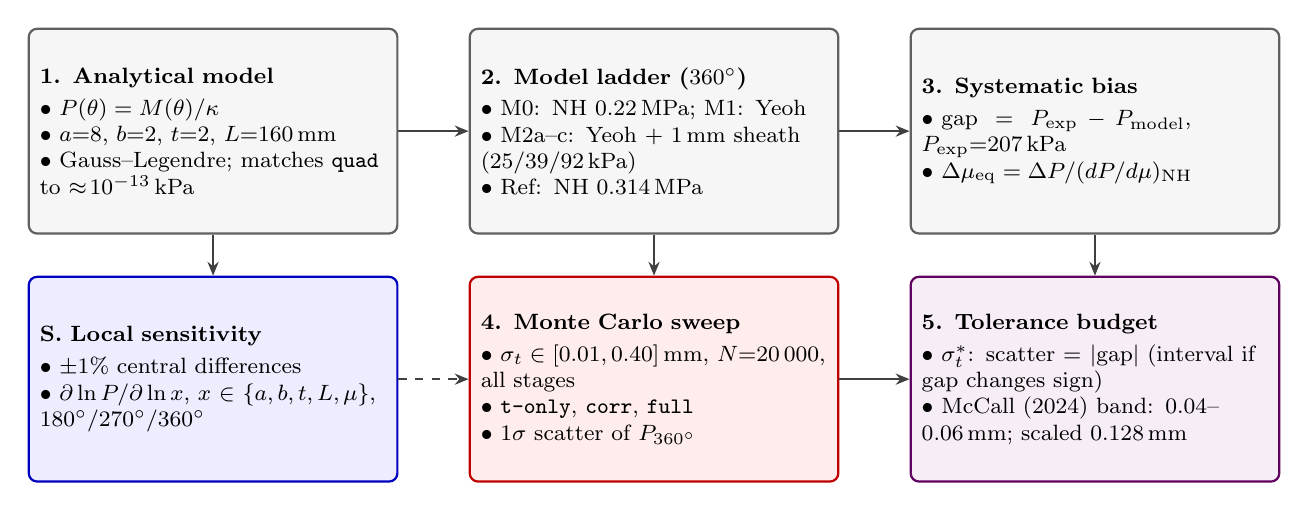
\begin{tikzpicture}[
    font=\footnotesize,
    box/.style={rectangle, rounded corners=3pt, draw=#1!75!black, fill=#1!7, line width=0.8pt,
                align=left, inner sep=4pt, text width=4.4cm, minimum height=2.6cm, anchor=north west},
    arr/.style={-{Stealth[length=5pt,width=4pt]}, line width=0.85pt, draw=black!75},
    dsh/.style={arr, dashed},
    ]
\newcommand{\bt}[1]{\textbf{#1}\\[2pt]}
% ---- row 1
\node[box=gray]  (model)  at (0,0)    {\bt{1. Analytical model}
  $\bullet$ $P(\theta)=M(\theta)/\kappa$\\
  $\bullet$ $a{=}8,\,b{=}2,\,t{=}2,\,L{=}160$\,mm\\
  $\bullet$ Gauss--Legendre; matches \texttt{quad} to $\approx\!10^{-13}$\,kPa};
\node[box=gray]  (ladder) at (5.6,0)  {\bt{2. Model ladder ($360^\circ$)}
  $\bullet$ M0: NH 0.22\,MPa; M1: Yeoh\\
  $\bullet$ M2a--c: Yeoh $+$ 1\,mm sheath (25/39/92\,kPa)\\
  $\bullet$ Ref: NH 0.314\,MPa};
\node[box=gray]  (bias)   at (11.2,0) {\bt{3. Systematic bias}
  $\bullet$ $\mathrm{gap}=P_{\mathrm{exp}}-P_{\mathrm{model}}$, $P_{\mathrm{exp}}{=}207$\,kPa\\
  $\bullet$ $\Delta\mu_{\mathrm{eq}}=\Delta P/(dP/d\mu)_{\mathrm{NH}}$};
% ---- row 2
\node[box=blue]  (sens)   at (0,-3.15)    {\bt{S. Local sensitivity}
  $\bullet$ $\pm1\%$ central differences\\
  $\bullet$ $\partial\ln P/\partial\ln x$, $x\in\{a,b,t,L,\mu\}$, $180^\circ$/$270^\circ$/$360^\circ$};
\node[box=red]   (mc)     at (5.6,-3.15)  {\bt{4. Monte Carlo sweep}
  $\bullet$ $\sigma_t\in[0.01,0.40]$\,mm, $N{=}20\,000$, all stages\\
  $\bullet$ \texttt{t-only}, \texttt{corr}, \texttt{full}\\
  $\bullet$ $1\sigma$ scatter of $P_{360^\circ}$};
\node[box=violet](budget) at (11.2,-3.15) {\bt{5. Tolerance budget}
  $\bullet$ $\sigma_t^{*}$: scatter $=|\mathrm{gap}|$ (interval if gap changes sign)\\
  $\bullet$ McCall (2024) band: 0.04--0.06\,mm; scaled 0.128\,mm};
% ---- arrows
\draw[arr]  (model.east |- ladder.east) -- (ladder.west);
\draw[arr]  (ladder.east) -- (bias.west);
\draw[arr]  (model.south) -- (sens.north);
\draw[arr]  (ladder.south) -- (mc.north);
\draw[dsh] (sens.east) -- (mc.west);
\draw[arr]  (mc.east) -- (budget.west);
\draw[arr]  (bias.south) -- (budget.north);
\end{tikzpicture}
\caption{Computational workflow: systematic bias (top row) vs.\ random tolerance scatter (bottom row) gives $\sigma_t^{*}$. Dashed: elasticities cross-check the Monte Carlo slope.}
\label{fig:workflow}
\end{figure}


\section{Results}
\textbf{Model ladder.} At $\mu_{\rm eff}=0.314$~MPa the model gives 237.8~kPa at $360^\circ$: 8.1\% above the 220~kPa quoted for the analytical model in Fig.~9 of \cite{poly2015} and 14.9\% above the measured 207~kPa. Table~\ref{tab:ladder} shows how the gap to 207~kPa shrinks along the ladder. Yeoh removes about 60\% of the Neo-Hookean gap; the sheath then flips its sign (zero at $\mu_s\approx30$~kPa).
\begin{table}[t]
\centering\small
\caption{Model ladder at $360^\circ$: pressure, gap to the measured 207~kPa, equivalent shift, crossover $\sigma_t^*$.}
\label{tab:ladder}
\begin{tabular}{lrrrrrrr}
\toprule
 & & & & \multicolumn{3}{c}{$\sigma_t^*$ (mm)}\\
\cmidrule(lr){5-7}
Stage & $P$ (kPa) & gap (kPa) & $\Delta\mu_{\rm eq}$ (MPa) & $t$ only & corr & full\\
\midrule
M0: NH, 0.22~MPa & 166.6 & $+40.4$ & $+0.053$ & 0.386 & 0.339 & 0.339\\
M1: Yeoh & 191.1 & $+15.9$ & $+0.021$ & 0.131 & 0.120 & 0.119\\
M2a: Yeoh + sheath 25~kPa & 204.3 & $+2.7$ & $+0.004$ & 0.022 & 0.020 & 0.013\\
M2b: Yeoh + sheath 39~kPa & 211.7 & $-4.7$ & $-0.006$ & 0.037 & 0.034 & 0.030\\
M2c: Yeoh + sheath 92~kPa & 239.7 & $-32.7$ & $-0.043$ & 0.246 & 0.218 & 0.218\\
\bottomrule
\end{tabular}
\end{table}

\textbf{Sensitivity.} At $360^\circ$ (Yeoh) the elasticities are $t$: $+1.27$, $L$: $-0.93$, $a$: $-0.45$, $b$: $+0.11$. \textbf{Crossover.} Fig.~\ref{fig:main}(a) and the last columns of Table~\ref{tab:ladder} give the main result. For the Yeoh reference ($|\text{gap}|=15.9$~kPa, equivalent to 0.021~MPa) $\sigma_t^*=0.13$~mm; the linearized formula gives 0.1308~mm against 0.1307~mm from the Monte Carlo. The measured band (0.04--0.06~mm) produces only 4.9--7.3~kPa of scatter, so bias dominates; the extrapolated upper end (0.128~mm) sits at the crossover. Fig.~\ref{fig:main}(b) shows $\sigma_t^*$ as a function of sheath stiffness: it falls from 0.13~mm at $\mu_s=0$ to zero at the sign change of the gap ($\mu_s\approx30$~kPa) and rises to 0.25~mm at 92~kPa. It is below the measured band (tolerance dominates) only for $\mu_s\approx21$--40~kPa (17--45~kPa against the upper end of the band); outside this window bias dominates. If the 8\% offset were real the window moves to $\mu_s\approx53$--72~kPa, which excludes the 25 and 39~kPa sheaths. Letting $a$ shift with $t$ (corr) raises the scatter by 9\% ($\sigma_t^*$ 0.131 to 0.120~mm); independent $a,b,L$ tolerances add a 2.3~kPa floor.


\begin{figure}[t]
\centering
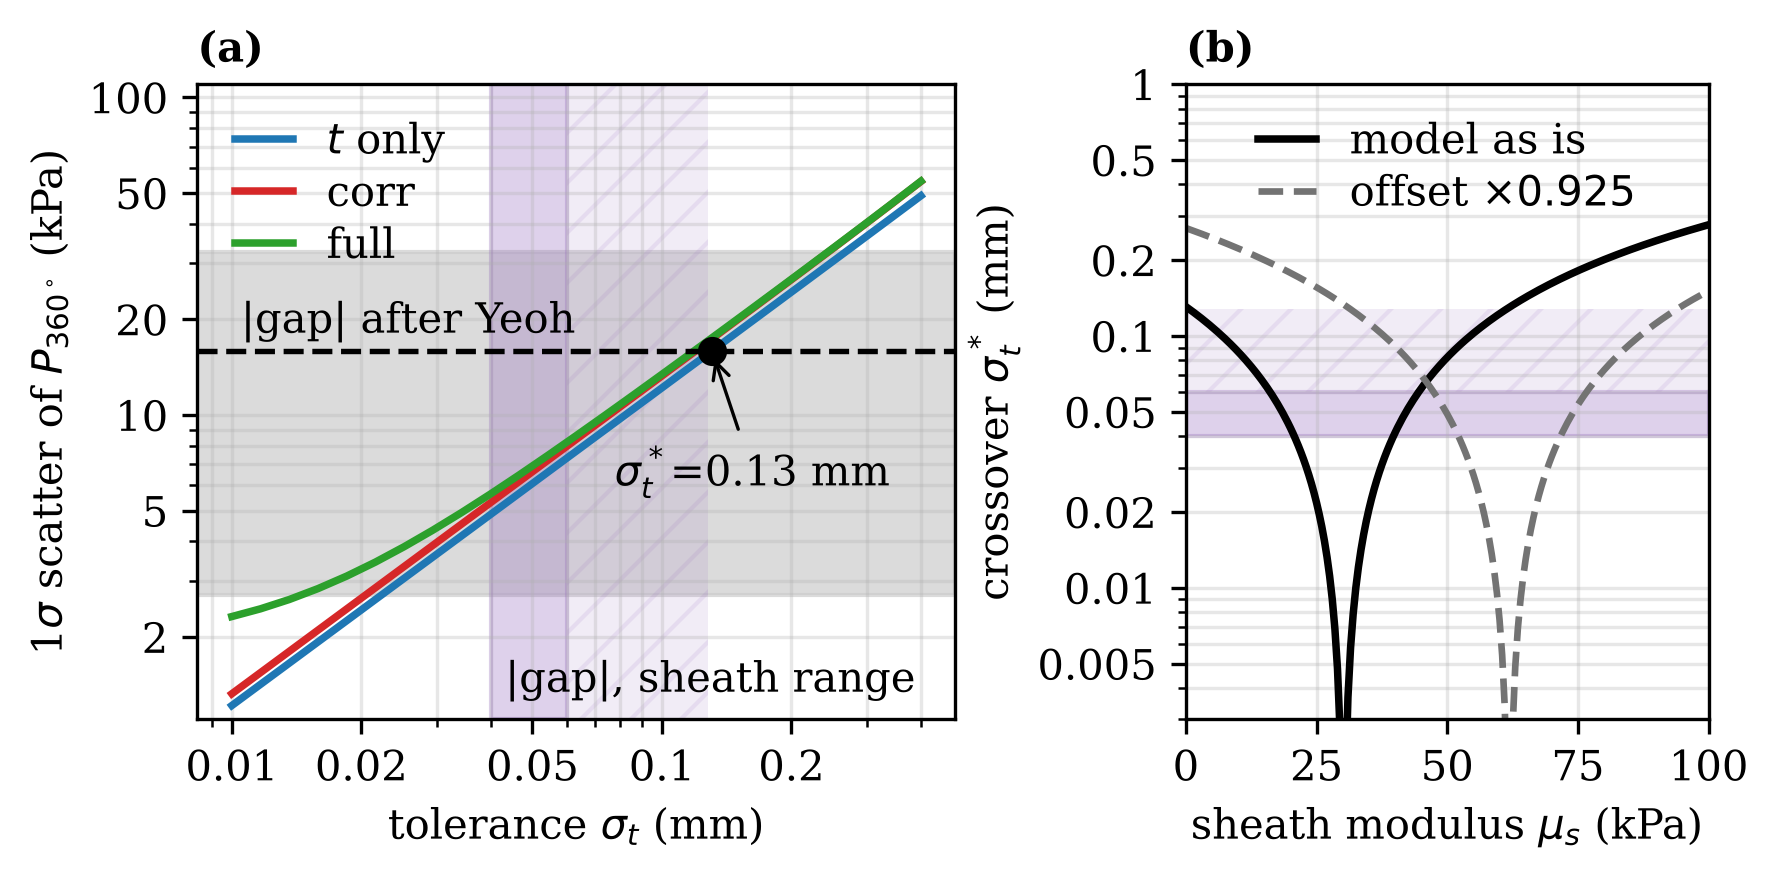
\includegraphics[width=\textwidth]{fig_main.png}
\caption{(a) $1\sigma$ scatter of $P_{360^\circ}$ (Yeoh) vs.\ $\sigma_t$ for $t$ only, corr and full. Dashed: $|\text{gap}|$ after Yeoh; gray: $|\text{gap}|$ over the sheath range. (b) $\sigma_t^*$ vs.\ sheath modulus (linearized), as is and with the 8\% offset. Purple: measured (dark) and extrapolated (hatched) tolerance \cite{mccall2024soft}.}
\label{fig:main}
\end{figure}

\section{Iteration and Future Work}
Three things changed during the project. (i)~The uniaxial Yeoh $I_1$ gave 186.8~kPa; the plane-strain form matching $\lambda-\lambda^{-3}$ gave 191.1~kPa. (ii)~The sweep started at 0.05~mm with a hypothesis range of 0.1--0.3~mm; the sheath-case crossovers (0.02--0.04~mm) showed both were too high, so it now starts at 0.01~mm and the hypothesis refers to the measured band. (iii)~My model follows Eqs.~14--19, 21 and the baseline of \cite{poly2015} but gives 237.8~kPa at $360^\circ$, 8\% above the analytical $\approx$220~kPa (consistent with the 10.9\% analytical-to-FEM error quoted there). Variants of stress law, width, moment arm, $\kappa$ and length did not explain it. A uniform 7.5\% offset (pressures and scatters $\times0.925$) would give $\sigma_t^*=0.27$, 0.16, 0.10, 0.12~mm for M1--M2c, so the result for the 25 and 39~kPa sheaths depends on it (Fig.~\ref{fig:main}b). \textbf{Limitations:} the sheath is fitted, not derived; the tolerance reference rests on three chambers thinner than 2~mm; one uniform $t$ per part; Fig.~10 not validated. \textbf{Next:} measure wall thicknesses; derive the sheath by FEM.

\section{Use of Generative AI}
\textbf{[CONFIRM and edit so this matches what you actually did.]} I used Claude (Anthropic) to help plan the project, draft the Python code and \LaTeX{} template, produce the figures, and check a cited paper's values against its PDF. I ran the code, checked the results against the course notebook and the model equations, and wrote or edited the final text myself.

\begin{thebibliography}{9}\small\setlength{\itemsep}{0pt}\setlength{\parskip}{0pt}
\bibitem{poly2015} P.~Polygerinos et al., ``Modeling of Soft Fiber-Reinforced Bending Actuators,'' \textit{IEEE Trans.\ Robot.}, 31(3):778--789, 2015.
\bibitem{mccall2024soft} J.~V. McCall, G.~D. Buckner, and D.~G. Kamper, ``Soft pneumatic actuators for pushing fingers into extension,'' \textit{J.\ NeuroEng.\ Rehabil.}, 21:146, 2024. doi:10.1186/s12984-024-01444-4.
\end{thebibliography}
\end{document}
